We begin by making one small change to the seq2seq modeling
framework. Instead of predicting the probability of the next
word, we instead learn to produce (non-probabilistic) scores
for ranking sequences. Define the score of a sequence consisting of 
\textit{history} $\pfx{t-1}$ followed by a single word $w_{t}$ as $f(w_{t}, \boldh_{t-1}, \boldx)$,
%\begin{align} \label{eq:score}
%\score(\pfx{t}, w_{t+1}) \triangleq f(w_{t+1}, \boldh_t, \boldx),
%\end{align} 
where $f$ is a parameterized function examining the current
hidden-state of the relevant RNN at time $t\,{-}\,1$ as well as the input
representation $\boldx$. In experiments, our $f$ will have an identical 
form to $g$ but \textit{without} the final softmax transformation (which transforms unnormalized scores into probabilities),  thereby allowing the model to avoid issues associated with the label bias
problem.

% employing a model that assigns
%a score to global sequences as opposed to probabilities to local
%decision avoids issues associated with the label bias
%problem

% Note that we use $\cdot$ as the concatenation
% operator. 

%As discussed in section~\ref{related}, employing a model that assigns
%a score to global sequences as opposed to probabilities to local
%decision avoids issues associated with the label bias
%problem. Unfortunately exactly computing gradients in standard
%sequence-level models requires performing an intractable search
%problem in training. [So his point here is that finding actual top K is infeasible; we can make the point that non-probabilistic loss allows us to not approximate] As seq2seq training is computationally very
%demanding to start, any major slowdown makes the training process
%infeasible.

More importantly, we also modify how this model is
trained. Ideally we would train by comparing the gold sequence to the
highest-scoring complete sequence. However, because finding the
argmax sequence according to this model is intractable, we
propose to adopt a LaSO-like~\cite{daume05learning} scheme to train, which we will refer to as beam search optimization (BSO). In particular, we define a loss that
penalizes the gold sequence falling off the beam during
training.\footnote{Using a non-probabilistic model further allows us
  to incur no loss (and thus require no update to parameters) when the
  gold sequence \textit{is} on the beam; this contrasts with models
  based on a CRF loss, such as those of \newcite{andor16globally} and
  \newcite{zhou15a}, though in training those models are simply not
  updated when the gold sequence remains on the beam.} The proposed
training approach is a simple way to expose the model to incorrect
histories and to match the training procedure to test
generation. Furthermore we show that it can be implemented efficiently
without changing the asymptotic run-time of training, beyond a factor
of the beam size $K$.

%Instead of directly optimizing our true loss,
%LaSO acknowledges that we will not be able to find the optimal target
%sequence even at test time. Therefore we instead train the model to
%correctly learn to rank sequences within beam search during training.


% using this model also requires a global training procedure. 



% of arbitrary \textit{sequences} formed from
% the target vocabulary $\mcV$. Weg will accordingly 


\subsection{Search-Based Loss}
We now formalize this notion of a search-based loss for RNN training. Assume we have a
set $S_t$ of $K$ candidate sequences of length $t$. We can calculate a
score for each sequence in $S_t$ using a scoring function $f$
parameterized with an RNN, as above, and we define the
sequence $\beampred{t}{K} \nicein S_t$ to be the $K$'th
ranked sequence in $S_t$ according to $f$. That is, assuming
distinct scores, 
\begin{align*}
\small
|\{ \beampred{t}{k} \nicein S_t \mid f(\hat{y}_t^{(k)}, \hat{\boldh}_{t-1}^{(k)}) > f(\hat{y}_t^{(K)}, \hat{\boldh}_{t-1}^{(K)})\}|
=
K\,{-}\,1,
\end{align*}
where $\hat{y}_t^{(k)}$ is the $t$'th token in $\beampred{t}{k}$,
$\hat{\boldh}_{t-1}^{(k)}$ is the RNN state corresponding to its
$t\,{-}\,1$'st step, and where we have omitted the $\boldx$ argument to $f$ for brevity. %$\beampred{t+1}{k}$ has a higher score than all but $k-1$ other sequences in $S_t$.
%That is (assuming all sequences in $\suk(\pfx{t})$ have distinct scores), we have 
%\begin{align*}
%|\{s \in \suk(\pfx{t}) \mid \score(s) > \score(\hat{\boldy}_{1:t+1}^{(k)})) \}| = k-1
%\end{align*}
%\mcL(f) =

We now define a loss function that gives loss each time the score of
the gold prefix $\goldpfx{t}$ does not exceed that of
$\beampred{t}{K}$ by a margin:
\begin{align*}
 \mcL&(f) = \\
 &\sum_{t=1}^T \Delta(\beampred{t}{K}) \left[1 - f(y_t, \boldh_{t-1}) + f(\hat{y}_t^{(K)},\hat{\boldh}_{t-1}^{(K)}) \right] .
\end{align*}
Above, the $\Delta(\beampred{t}{K})$ term denotes a
mistake-specific cost-function, which allows us to scale the loss
depending on the severity of erroneously predicting $\beampred{t}{K}$;
it is assumed to return 0 when the margin requirement is satisfied,
and a positive number otherwise. It is this term that allows us to use sequence- rather than word-level costs in training (addressing the 2nd issue in the introduction). For instance, when training a seq2seq model for machine translation, it may be desirable to have $\Delta(\beampred{t}{K})$ be inversely related to the partial sentence-level BLEU score of $\beampred{t}{K}$ with $\goldpfx{t}$; we experiment along these lines in Section~\ref{sec:tasks}. 

Finally, because we want the full gold sequence to be at the top of the beam at the end of search, when $t \niceq T$ we modify the loss to require the score of $\goldpfx{T}$ to exceed the score of the \textit{highest} ranked incorrect prediction by a margin.

We can optimize the loss $\mcL$ using a two-step process: (1) in a forward pass, we compute candidate sets $S_t$ and record margin violations (sequences with non-zero loss); (2) in a backward pass, we back-propagate the errors through the seq2seq RNNs.
%\begin{itemize}
%\item compute candidate sets $S_t$ and collect losses 
%\item back-propagate the errors through the seq2seq RNNs and update the parameters 
%\end{itemize}
Unlike standard seq2seq training, the first-step requires running
search (in our case beam search) to find margin violations. The second
step can be done by adapting back-propagation through time (BPTT). 
We next discuss the details of this process.


% The first-step requires the 

% \textbf{[When is the right time to note that at the final step we require gold to actually be first on beam?]}

\subsection{Forward: Find Violations} 
\label{sec:forward}
In order to minimize this loss, we need to specify a procedure for
constructing candidate sequences $\beampred{t}{k}$ at each time step
$t$ so that we find margin violations. We follow LaSO (rather than
early-update \footnote{We found that training with early-update rather than (delayed)
LaSO did not work well, even after pre-training. Given the success of early-update
in many NLP tasks this was somewhat surprising. We leave this question to future work.}; see Section~\ref{sec:relatedwork}) and build candidates
in a recursive manner. If there was no margin violation at $t{-}1$,
then $S_t$ is constructed using a standard beam search update. If
there was a margin violation, $S_t$ is constructed as the $K$ best
sequences assuming the gold history $y_{1:t-1}$ through time-step $t{-}1$.

%  that violate this
% margin criteria. To do this calculate $\beampred{t}{K}$ at each
% time-step $t$ with respect to the set $S_t$ consisting of candidate
% sequences of length $t$ that can be formed from the $K$ highest
% scoring sequences generated at the $t\,{-}\,1$'st step of beam-search
% \textit{if we incurred no loss at time $t\,{-}\,1$}; otherwise $S_t$
% consists of only those candidates that can be formed from
% $\goldpfx{t}$. 

Formally, assume the
function $\suk$ maps a sequence $\pfx{t-1} \nicein \mcV^{t-1}$ to the
set of all valid sequences of length $t$ that can be formed by appending to it a
valid word $w \nicein \mcV$. In the
simplest, unconstrained case, we will have
\begin{align*}
\suk(\pfx{t-1}) = \{\pfx{t-1}, w \mid w \in \mcV \}.
\end{align*}

As an important aside, note that for some problems it may be preferable to define a
$\suk$ function which imposes hard constraints on successor sequences. For instance, if we would like to use seq2seq models for parsing (by emitting a constituency or dependency structure encoded into a sequence in some way), we will have hard constraints on the sequences the model can output, namely, that they represent valid parses. While hard constraints such as these would be difficult to add to standard seq2seq at training time, in our framework they can naturally be added to the $\suk$ function, allowing us to \textit{train} with hard constraints; we experiment along these lines in Section~\ref{sec:tasks}, where we refer to a model trained with constrained beam search as ConBSO. 

Having defined an appropriate $\suk$ function, we specify the candidate set as: 
\begin{align*} \label{eq:stupdate}
S_t =  \topK\begin{cases}  \suk(\goldpfx{t-1}) &\mbox{violation at } t{-}1\\
\bigcup_{k=1}^K \suk(\beampred{t-1}{k}) &\mbox{otherwise}, \end{cases}
\end{align*}
where we have a margin violation at $t{-}1$ iff $f(y_{t-1}, \boldh_{t-2}) < f(\hat{y}_{t-1}^{(K)},\hat{\boldh}_{t-2}^{(K)}) + 1$, and where $\topK$ considers the scores given by $f$. This search procedure is illustrated in the top portion of Figure~\ref{fig:backprop}. 

In the forward pass of our training algorithm, shown as the first part of Algorithm~\ref{alg:treebp}, we run this version of
beam search and collect all sequences and their hidden states that
lead to losses. 

\begin{figure}[t!]
\centering
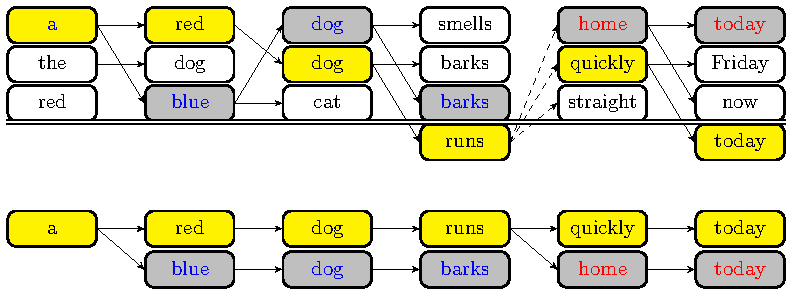
\includegraphics[width=1\columnwidth]{beam}
\caption{Top: possible $\beampred{t}{k}$ formed in training with a beam of size $K \niceq 3$ and with gold sequence $\goldpfx{6}$ = ``a red dog runs quickly today''. The gold sequence is highlighted in yellow, and the predicted prefixes involved in margin violations (at $t \niceq 4$ and $t \niceq 6$) are in gray. Note that time-step $T \niceq 6$ uses a different loss criterion. Bottom: prefixes that actually participate in the loss, arranged to illustrate the back-propagation process.}
\label{fig:backprop}
\end{figure}


\subsection{Backward: Merge Sequences}
Once we have collected margin violations we can run backpropagation to compute parameter updates. Assume a
margin violation occurs at time-step $t$ between the predicted history
$\beampred{t}{K}$ and the gold history $\goldpfx{t}$. As in standard
seq2seq training we must back-propagate this error through the gold
history; however, unlike seq2seq we also have a gradient for the
wrongly predicted history.

Recall that to back-propagate errors through an RNN we run a recursive backward procedure --- denoted below by $\BRNN$ --- at each time-step $t$, which accumulates the 
gradients of next-step and future losses with respect to $\boldh_t$. We have: 
\begin{align*}
\nabla_{\boldh_t} \mcL \gets \BRNN(\nabla_{\boldh_t} \mcL_{t+1},\nabla_{\boldh_{t+1}} \mcL),
\end{align*} 
where $\mcL_{t+1}$ is the loss at step $t \, {+} \, 1$, deriving, for instance, from the score $f(y_{t+1}, \boldh_{t})$.
%\begin{align*}
%\nabla_{\boldh_t} \mcL \gets \nabla_{\boldh_t} \mcL + \BRNN(\nabla_{\boldh_{t+1}} \mcL, \boldm_t, \boldh_{t}).
%\end{align*}
%Note that $\boldm_t$ is the embedding corresponding to output word $w_t$. 
Running this $\BRNN$ procedure from $t \niceq T \, {-} \,1$ to $t \niceq 0$ is known as back-propagation through time (BPTT).

In determining the total computational cost of back-propagation here, first note that in the worst case there is one violation at each time-step, which
leads to $T$ independent, incorrect sequences. Since we need to call $\BRNN$
$O(T)$ times for each sequence, a naive strategy of running BPTT for each incorrect sequence would lead to an $O(T^2)$ backward pass, rather than the $O(T)$ time required for the standard seq2seq approach. 

Fortunately, our combination of search-strategy and loss make it
possible to efficiently share $\BRNN$ operations. This shared
structure comes naturally from the LaSO update, which resets the beam in a convenient way. 


% Note though that this differs from standard 
% seq2seq training in that we have gradients for   


% Using this search procedure

% An online implementation of the training scheme implied by the loss
% and search-strategy discussed above would then involve beam-searching
% in linear order for the target sequence, using \eqref{eq:stupdate} to
% determine the set of candidates $S_t$ at each time-step. If a margin
% violation occurs at time-step $t$, errors would then be backpropagated
% through both the predicted prefix $\beampred{t}{K}$ and the gold
% prefix $\goldpfx{t}$. The problem with such an approach, however, is
% that it has a worst-case quadratic dependence on $T$, the length of
% the target sequence, since it backpropagates for every violating
% prefix. 

We informally illustrate the process in Figure~\ref{fig:backprop}. The
top of the diagram shows a possible sequence of $\beampred{t}{k}$
formed during search with a beam of size 3 for the target sequence
$y=$ ``a red dog runs quickly today.'' When the gold sequence falls
off the beam at $t \niceq 4$, search resumes with
$S_5 \niceq \suk(\goldpfx{4})$, and so all subsequent predicted
sequences have $\goldpfx{4}$ as a prefix and are thus functions of
$\boldh_4$. Moreover, because our loss function only involves the
scores of the gold prefix and the violating prefix, we end up with the
relatively simple computation tree shown at the bottom of
Figure~\ref{fig:backprop}. It is evident that we can backpropagate
in a single pass, accumulating gradients from sequences that diverge
from the gold at the time-step that precedes their divergence. The
second half of Algorithm~\ref{alg:treebp} shows this explicitly for a
single sequence, though it is straightforward to extend the algorithm
to operate in batch.\footnote{We also note that because
  we do not update the parameters until after the $T$'th search step, our training procedure
  differs slightly from LaSO (which is online), and in this aspect is
  essentially equivalent to the ``delayed LaSO update'' of \newcite{BandK:14}.}
{\small
\begin{algorithm}[t!]
  \small
  \begin{algorithmic}[1]
    \Procedure{BSO}{$\boldx, K_{tr}, \suk$}
    \State{/*\textsc{Forward}*/}
    \State{Init empty storage $\hat{y}_{1:T}$ and $\hat{\boldh}_{1:T}$; init $S_1$}
    \State{$r \gets 0$; $violations \gets \{0\}$}
    \For{$t=1,\ldots,T$}
    \State{$K \niceq K_{tr}$ if $t \, {\neq} \,T$ else $\displaystyle \argmax_{k: \beampred{t}{k} \neq \goldpfx{t}} {\footnotesize f(\hat{y}_t^{(k)}, \hat{\boldh}_{t-1}^{(k)})}$}
    \If{$f(y_{t}, \boldh_{t-1}) < f(\hat{y}_t^{(K)},\hat{\boldh}_{t-1}^{(K)}) + 1$}  
    \State{$\hat{\boldh}_{r:t-1} \gets \hat{\boldh}^{(K)}_{r:t-1}$}
    \State{$\hat{y}_{r+1:t} \gets \hat{y}^{(K)}_{r+1:t}$}    
    \State{Add $t$ to $violations$}
    \State{$r \gets t$}
    \State{$S_{t+1} \gets \topK(  \suk(\goldpfx{t}))$}
    \Else{}
    \State{$S_{t+1} \gets \topK( \bigcup_{k=1}^K \suk(\beampred{t}{k})) $}
    \EndIf{}
    
    \EndFor{}
    \State{/*\textsc{Backward}*/}
%    \State{$\nabla_{\boldh_T} \gets - \Delta(\beampred{T}{K}) \times \nabla_{\boldh_T} f(\goldpfx{T})$}    
%    \State{$\nabla_{\widehat{\boldh}_T} \gets \Delta(\beampred{T}{K}) \times \nabla_{\widehat{\boldh}_T} f(\beampred{T}{K})$}    
%    \State{$\nabla_{\boldh_{T}} \gets \bzero$; $\nabla_{\widehat{\boldh}_{T}} \gets \bzero$}
    \State{$grad\_{\boldh_{T}} \gets \bzero$; $grad\_{\widehat{\boldh}_{T}} \gets \bzero$}
    \For{$t=T-1,\ldots,1$}
    \State{$grad\_{\boldh_t} \, {\gets} \, \BRNN(\nabla_{\boldh_t} \mcL_{t+1}, grad\_{\boldh_{t+1}})$
      }
    \State{$grad\_{\widehat{\boldh}_t} \, {\gets} \, 
    \BRNN(\nabla_{\widehat{\boldh}_t} \mcL_{t+1}, grad\_{\widehat{\boldh}_{t+1}})$
      }      

    \If{$t \, {-} \, 1 \in violations$}
    \State{$grad\_{\boldh_t} \gets grad\_{\boldh_t} + grad\_{\widehat{\boldh}_t}$}     
    \State{$grad\_{\widehat{\boldh}_t} \gets \bzero$ }
    \EndIf{}
    \EndFor{}
    %\State{Update RNN params based on $\boldh, \hat{\boldh}$ }
    \EndProcedure{}
  \end{algorithmic}
  \caption{\label{alg:treebp} Seq2seq Beam-Search Optimization}
\end{algorithm}
}
  
%  {\small
%\begin{algorithm}[t!]
%  \small
%  \begin{algorithmic}[1]
%    \Procedure{BSOTrain}{$K_{tr}$}
%    \State{/*\textsc{Forward}*/}
%    \State{Init empty $\hat{y}_{1:T}$ and $\hat{\boldh}_{1:T}$; init $S_1$}
%    \State{$resets \gets [0]$}
%    \For{$t=1,\ldots,T$}
%    \State{$K \niceq K_{tr}$ if $t \, {\neq} \,T$ else $\displaystyle \argmax_{k: \beampred{t}{k} \neq \goldpfx{t}} {\footnotesize f(\beampred{t}{k}, \hat{\boldh}_{t-1}^{(k)})}$}
%    \If{$f(y_{t}, \boldh_{t-1}) < f(\hat{y}_t,\hat{\boldh}_{t-1}^{(K)}) + 1$}  
%   
%    \State{$r \gets top(resets)$}
%    \State{$\hat{\boldh}_{r:t-1} \gets \hat{\boldh}^{(K)}_{r:t-1}$}
%    \State{$\hat{y}_{r+1:t} \gets \hat{y}^{(K)}_{r+1:t}$}    
%    \State{Push $t$ onto $resets$}
%    \State{$S_{t+1} \gets \topK(  \suk(\goldpfx{t}))$}
%    \Else{}
%    \State{$S_{t+1} \gets \topK( \bigcup_{k=1}^K \suk(\beampred{t}{k})) $}
%    \EndIf{}
%    
%    \EndFor{}
%    \State{/*\textsc{Backward}*/}
%    %\State{Zero gradients $\nabla_{\boldh_1}, \ldots,\nabla_{\boldh_T}, \nabla_{\widehat{\boldh}_1}, \ldots, \nabla_{\widehat{\boldh}_T}$}
%    \State{$\nabla_{\boldh_T} \gets - \Delta(\beampred{T}{K}) \times \nabla_{\boldh_t} f(\goldpfx{T})$}    
%    \State{$\nabla_{\widehat{\boldh}_T} \gets \Delta(\beampred{T}{K}) \times \nabla_{\widehat{\boldh}_t} f(\beampred{T}{K})$}    
%    \For{$t=T-1,\ldots,1$}
%    \State{$\nabla_{\boldh_t} \gets 
%        \BRNN(y_{t+1}, \boldh_{t},\nabla_{\boldh_{t+1}})$ 
%        \\ $\qquad \qquad \qquad   - \Delta(\beampred{t}{K}) \times \nabla_{\boldh_t} f(\goldpfx{t})$
%      }
%    \State{$\nabla_{\widehat{\boldh}_t} \gets 
%        \BRNN(\hat{y}_{t+1}, \hat{\boldh}_{t},\nabla_{\widehat{\boldh}_{t+1}})$ \\ $\qquad \qquad \qquad   + \Delta(\beampred{t}{K}) \times \nabla_{\widehat{\boldh}_t} f(\beampred{t}{K})$
%      }      
%
%    \If{$t \, {-} \, 1 \in resets$}
%    \State{$\nabla_{\boldh_t} \gets \nabla_{\boldh_t} + \nabla_{\widehat{\boldh}_t}$}     
%    \State{$\nabla_{\widehat{\boldh}_t} \gets \bzero$ }
%    \EndIf{}
%   
%    
%    \EndFor{}
%    \State{Update RNN params based on $\boldh, \boldh', \hat{\boldh}, \hat{\boldh}'$ }
%    \EndProcedure{}
%  \end{algorithmic}
%  \caption{\label{alg:treebp} Seq2seq Beam-Search Optimization}
%\end{algorithm}
%}

 
 
  
%{\small
%\begin{algorithm}[t!]
%  \begin{algorithmic}[1]
%    \Procedure{Train}{$beamsize$, $S_1$}
%    \State{$last, grad, \hat{y}, \hat{\boldh}_{1:T} \gets 0, \{\}, \{\}, \{\}$}
%    \For{$t=1,\ldots,T$}
%    \State{$K = beamsize$ if $t\neq T$ else 1 }
%    % \State{Find $\beampred{t}{K}$ wrt $S_t$}
%    \If{$f(y_{t}, \boldh_{t-1}) < f(\hat{y}_{t}^{(K)},\hat{\boldh}_{t-1}^{(K)}) + 1$}  
%    
%    \State{$grad[t] = $ grad of loss wrt f}     
%
%    \State{$\hat{\boldh}_{last:t-1} \gets \hat{\boldh}^{(K)}_{last:t-1}$}
%    \State{$\hat{y}_{last:t} \gets \hat{y}^{(K)}_{last:t}$}
%%    \State{Backprop $\Delta(\beampred{t}{K})$ through $\beampred{t}{K}$} 
%%    \State{Backprop $-\Delta(\beampred{t}{K})$ through $\goldpfx{t}$}     
%    \State{$last \gets t +1$}
%    \State{$S_{t+1} \gets \topK(  \suk(\goldpfx{t}))$}
%    \Else{}
%    \State{$S_{t+1} \gets \topK( \bigcup_{k=1}^K \suk(\beampred{t}{k})) $}
%    \EndIf{}
%    
%    \EndFor{}
%    \State{Define gradients $\boldh'_{1:T}$, $\hat{\boldh}'_{1:T}$}
%    \State{$\boldh'_{T+1} \gets 0$, $\hat{\boldh}'_{T+1} \gets 0$ }
%    \For{$t=T,\ldots,1$}
%    \State{$\boldh'_{t} \gets \BRNN(\boldh'_{t+1}, y_{t+1}, \boldh_{t}) $}
%    \If{$t \in grad$}
%    % \State{\Comment{Merge last violation}}
%    \State{$\boldh'_{t} \gets \boldh'_{t} + \BPTT(\hat{\boldh}'_{t+1}, y_{t+1}, \hat{\boldh}_{t}) $}     
%
%    % \State{\Comment{New gradient from loss}}
%    \State{$\boldh'_{t} \gets \boldh' - grad[t]$ }
%    \State{$\hat{\boldh}'_{t} \gets grad[t]$ }
%    % \State{$\boldh'_{t} \gets \boldh'_{t} + BPTT(\boldh'_{t},\boldh_{t-1}) $}
%    % \State{Backprop $\Delta(\beampred{t}{K})$ through $\beampred{t}{K}$} 
%    \Else{}
%    % BPTT new guy
%    \State{$\hat{\boldh}'_{t} \gets  \BPTT(\hat{\boldh}'_{t+1},\hat{y}_{t+1}, \hat{\boldh}_{t}) $}     
%    \EndIf{}
%    % \State{$\boldh'_{t-1} \gets BPTT(\boldh'_{t},\boldh_{t-1})$} 
%    % \State{$\boldh_{t-1} \gets BPTT(\boldh'_{t},\boldh_{t-1})$} 
%    % \State{Backprop $-\Delta(\beampred{t}{K})$ through $\goldpfx{t}$}     
%    
%    \EndFor{}
%    \State{Update RNN params based on $\boldh, \boldh', \hat{\boldh}, \hat{\boldh}'$ }
%    \EndProcedure{}
%  \end{algorithmic}
%  \caption{\label{alg:treebp} seq2seq Beam-Search Optimization}
%\end{algorithm}
%}


% \textbf{Not sure where this goes, but not here}
% We pause to note some of the benefits of the proposed approach. In doing so,  we distinguish between the model itself and the way it is trained. Beginning with the model, we note that it does not suffer from label bias, since it scores entire prefixes rather than words. Furthermore, setting $\Delta$ appropriately allows the model to be sensitive to sequence-level costs during training. The training procedure, on the other hand, tackles exposure bias, since the model must learn to rank the gold prefix higher than its own predictions generated through search. Finally, the training procedure also allows for enforcing hard-constraints during training, since we may define a more complicated $\suk$ function, which requires $S_t$ to contain only sequences satisfying certain constraints. This idea opens the possibility of doing feasible-set training with RNNs. We explore these ideas further in Section~\ref{sec:experiments}.

